\chapter{Design möglicher Aggregationsschnitte }

Ein Domainmodell kann auf unterschiedliche Weise realisiert werden. Dies gilt ebenfalls für den Schnitt der Aggregates. Verschiedene Gruppierungen genießen zugleich andere Vor- und Nachteile. In diesem Kapitel werden mehrere mögliche Aggregationsaufteilungen untersucht und anhand von Kriterien, wie unter anderem Performance, Komplexität, Parallelität, Anwendbarkeit und Client-Freundlichkeit, bewertet.

\section{Ein zusammengehöriges Basket-Aggregate als initiales Design}

Das Design eines großen Aggregates fällt Entwicklern meist einfacher. Bei einer einzelnen, zusammenhängenden Struktur, durch welche unmittelbar Daten bearbeitet und Invarianten überprüft werden können, hält sich die Komplexität weitestgehend in Grenzen. Vor allem müssen kaum Überlegungen über die transaktionale Konsistenz getroffen werden, da die Transaktion das gesamte Datenmodell umspannend. Die erste Variante des Proof-of-Concepts wurde mit diesem Design in Gedanken entwickelt und stellt das Grundgerüst für alle kommende Ansätze dar. Dementsprechend ist der Basket hier das Aggregate Root und alle verbleibenden Klassen sind diesem unterteilt. Zur vereinfachten Referenz auf die einzelnen Umsetzungsmöglichkeiten wird das Design als '\emph{Variante A}' betitelt.


\subsection{Performance von unterschiedlich großen Aggregates im Vergleich}

Als Konsequenz eines umfassenderen Aggregates muss immer die gesamte Datenstruktur geladen werden, da auf darunterliegende Objekte nur durch das Aggregate Root zugegriffen werden darf. Für die Aktualisierung von Attributen tief im Aggregat müssen somit alle anderen Daten ebenfalls aus der Datenbank gelesen werden. Die Auswirkungen dieser Tatsache kann mithilfe von \gls{Lazy Loading} oder durch Einsatz einer dokumentenorientierten Datenbank eingeschränkt werden. Generell gilt, dass große Aggregates aus Sicht der Performance langsamer arbeiten als kleinere. Diese Aussage ist allerdings mit Vorsicht zu genießen und kann je nach Anwendungsgebiet sogar gegensätzlich ausfallen. In diesem Unterkapitel wird diese Richtlinie anhand des vorliegenden Bounded-Contexts analysiert.

\textbf{Untergliederung des Baskets in kleinere Bestandteile}

Wie oben erwähnt, ermöglicht ein kleinerer Aggregationsschnitt das unabhängige Laden und Bearbeiten der Aggregates. In Betrachtung der Anwendungsfälle beziehen sich Aktionen meist auf einzelne Value Objects, Basket-Items oder den Payment-Process. Dementsprechend wäre das explizite Abfragen dieser Daten aus der Datenquelle effektiver. Dies ist in Domain-Driven Design jedoch nur möglich, sofern diese Klassen die Rolle eines Aggregate Root einnehmen. Wird die \emph{Variante A} unterteilt in ein Basket-, Payment und Basket-Item-Aggregate (\emph{'Variante B'}) können sie somit unabhängig voneinander gehandhabt werden. Eine kurze Übersicht über diesen neuen Aggregationsschnitt bietet Abbildung \ref{fig:VarB}. Ohne Beachtung, welche Auswirkungen dieses neu überlegte Design auf andere Faktoren hat, ist eine erhöhte Performance anhand erster Überlegungen zu erwarten. Die vermeintlich gewonnene Leistungsverbesserung wird allerdings aufgrund folgender Umstände minimiert.

\begin{figure}[htbp]
	\centering
	\includesvg[inkscapelatex=false, width=0.80\textwidth]{svg/VarB.svg}
	\caption{Aggregationsschnitt der Variante B}
	\label{fig:VarB}
\end{figure}

\vspace{1em}

\textbf{Invarianten über Aggregationsgrenzen hinweg}

Wird dem Warenkorb ein neuer Artikel hinzugefügt, hat dies nicht nur das Anlegen eines Items, sondern auch die Neukalkulation des Baskets zur Folge. Sofern eine Trennung zwischen Basket und Basket-Item vorliegt, müssen dennoch alle Items aus der Datenbank geladen werden, andernfalls ist es nicht möglich den neuen Gesamtpreis zu ermittelt. Innerhalb eines Checkout-Kontextes existieren viele dieser klassenübergreifenden Businessanforderungen, weshalb die Kopplung des Datenmodells oftmals eine wirklich unabhängige Datenanpassung eines Aggregates in \emph{Variante B} verhindert.

Durch eine genauere Untersuchung der Anwendungsfälle kann eine Abwägung getroffen werden, wie viele Prozesse tatsächlich isoliert abzuarbeiten sind. Die Effektivität des Aggregationsdesigns ist ebenfalls an die Bedürfnisse der Clients gekoppelt sind. Sofern diese bei einem API-Aufruf den vollständigen Warenkorb als Antwort erwarten, muss auch hier ein aggregationsübergreifender Ladevorgang stattfinden. Das Stornieren des Baskets und Setzten der Checkout-Daten ist hingegen positiv von dieser Anpassung betroffen, denn diese verwaltet alleinig der Warenkorb. Die meisten API-Anfragen beziehen sich allerdings auf beinhaltete BasketItems und die Verwaltung des Bezahlvorgangs, welche Wechselwirkungen mit dem Warenkorb oder sein zugehöriger Gesamtpreis besitzen. Letztendlich sind nur eine Bruchzahl der Anwendungsfälle mithilfe von Variante B unabhängig abschließbar, somit steigt die Anzahl der benötigten Datenbankoperationen auch bei kleineren Aggregates und die damit verbundene Bearbeitungszeit wieder an.

In dem Buch '\citetitle{Evans.2011}' wird zusätzlich auf eine Richtlinie hingewiesen, dass bei korrekten Aggregationsdesign eine Transaktion maximal ein Aggregate bearbeiten sollte \cite[S. 354]{Evans.2011}. Dies führt zu einem Konflikt mit den vorgehenden Businessanforderungen. Beispielsweise wäre es nicht möglich bei der Initiierung des Zahlungsvorgangs zeitgleich den Warenkorb einzufrieren. Ein möglicher Lösungsansatz stellt hierbei das Verwenden von eventueller Konsistenz dar. Konkret findet die Bearbeitung der Aggregates zeitversetzt voneinander statt, weshalb eine Zeitspanne existiert in welcher der Datensatz einen invaliden Stand besitzt. Angewandt an den vorgehenden Anwendungsfall bedeutet dies, dass zwar der Warenkorb eingefroren, allerdings der Bezahlvorgang noch nicht gestartet ist. Verbundene Implikationen mit eventueller Konsistenz werden in einem folgenden Kapitel besprochen.

\subsubsection{Einfluss des verwendeten Datenbanksystems auf den Aggregationsschnitt}

Das Design einer Software soll stets, so weit wie möglich, abgekapselt von verwendeten Technologien sein. Technologien entwickeln sich weiter, werden durch neuer ersetzt und bringen unnötige Abhängigkeiten in den Quelltext. Theoretisch hat somit eine Beeinflussung der Architektur durch eine externe Komponente einen negativen Effekt auf die Qualität der Software und ihre Wartbarkeit. Dennoch kann in der Praxis dieser Gedanke durchaus Vorteile bergen, welche dieses Vorgehen rechtfertigt. Deshalb wird im folgenden Abschnitt das Aggregationsdesign aus Sicht der Datenbank bewertet.

Laut Definition erhält jedes Aggregate bzw. Aggregate Root eine eigene Tabelle in der darunterliegenden, relationalen Datenbank. Deshalb existiert in \emph{Variante B} mindestens eine Tabelle für den Basket, Basket-Items und Payment-Process. Hingegen kann bei \emph{Variante A} der Payment-Process in die Basket-Tabelle hinzugefügt werden, da eine Eins-zu-Eins Relation vorliegt. Weitergehend benötigen beide Aggregationsschnitte aufgrund der Eins-zu-N Beziehung zwei Tabellen für Basket und Basket-Item. Dementsprechend muss beim Abruf eines kompletten Baskets in \emph{Variante A} im Vergleich zu \emph{Variante B} weniger Ladevorgänge durchgeführt werden. Das kleiner Aggregationsdesign ist bei isolierten Modifikationen von Aggregates aus Sicht der Datenbankoperationen jedoch vorteilhafter. Je nach Businessanforderungen können sich diese Aspekte ausgleichen und lediglich einen geringen Effekt auf die generelle Performance der Anwendung besitzen.

Sollte die verwendete Datenbank allerdings einen dokumentenorientierten Ansatz verfolgen, gilt vorheriger Absatz nur noch bedingt. Hierbei benötigt \emph{Variante B} weiterhin pro Aggregate eine eigene \gls{Collection}. \emph{Variante A} kann das komplette Datenmodell hingegen in einem einzigen Eintrag persistierten. An sich ist der einzelne Datensatz umfangreicher, allerdings durch die eingesparten Datenbankoperationen dennoch effektiver. Daher würde bei einem Umbau der Aggregates für die meisten Anwendungsfälle eine einzelne Suchanfrage in mehrere abgewandelt werden, wodurch bemerkbare Auswirkungen auf die Antwortzeit der Applikation entstehen können. 

Anfangs wurde beschrieben, dass eine Technologie idealerweise keine Auswirkung auf die Architektur haben sollte, konträr dazu ist bei der Betrachtung der Applikationsperformance dies eventuell sinnvoll. Sollte eine relationale Datenbank verwendet werden, hält sich die Performance-Unterschiede in Grenzen, wohingegen dies bei einen umfangreicher Aggregationsschnitt mit einer dokumentenorientierten Datenbank nicht gewährleistet werden kann. Anhand eines konkreten Lasttests wird in einem späteren Kapitel dieser Effekt genauer untersucht und bewertet.

\subsection{Parallele Bearbeitung eines großen Aggregates}

Ausgehend von \emph{Variante A} resultiert eine Bearbeitung des Baskets in der Speicherung des kompletten Warenkorbs in der Datenbank. Bei Schreibprozessen können Anomalien auftreten, wodurch die Operation abgebrochen werden muss. Eine mögliche Anomalie ist das sogenannte 'Lost Update'-Problem. Es kann auftreten, wenn zwei Transaktionen den gleichen Datensatz zeitgleich bearbeiten. Anfangs besitzen beide denselben Startzustand, jedoch beim Zurückschreiben ihrer Ergebnisse stößt der letztere von beiden auf einen nun neueren Stand. Hierbei muss diese Transaktion erkannt und abgebrochen werden, da sonst die zuvor geschehene Datenänderung der ersteren Transaktion verloren gehen würde.

Konkretisiert kann dieses Problem auftreten, wenn beispielsweise zwei Personen einen neuen Artikel dem gleichen Warenkorb hinzufügen. Der erste Kunde legt hierbei ein neues Handy in den Warenkorb, wohingegen zeitgleich ein anderer Nutzer einen Fernseher hinzufügt. Beide Transaktionen starten mit einem leeren Warenkorb und schreiben in die Datenbank einen Datensatz mit nur einem Artikel. Das System aktualisiert den Eintrag in der Datenbank zuerst mit dem Handy. Aufgrund dessen, dass die zweite Anfrage mit einem leeren Warenkorb initiiert worden ist, wird der Datensatz ebenfalls mit nur einen Artikel persistiert. Letztendlich enthält der Basket nun nur einen Fernseher statt den eigentlichen zwei Artikeln. Alternativ kann die letztere Operation anhand des neuen Zustandes erneut durchgeführt werden oder der Datensatz wird beim Laden für weitere Anfragen gesperrt, sodass ein solches Problem nicht auftreten kann. Diese Lösungsansätze nennen sich optimistisches bzw. pessimistisches Sperrverfahren. 

Innerhalb eines großen Aggregates kann es bei zeitgleichen Aktionen vermehrt zu Schreibanomalien kommen, wodurch sie sich für parallele Bearbeitung nicht eigenen. In \emph{Variante B} ist es möglich Basket-Items zum selben Zeitpunkt anzupassen, da sie in der Datenbank unabhängig voneinander persistiert werden. Existieren Businessanforderungen für Ressourcen, welche mehrere Nutzer gleichzeitig verwalten, ist ein umfassenderer Aggregationsschnitt nur noch bedingt möglich. Deswegen muss vor dem Entwicklungsprozess bei der Aufnahme des Funktionsumfanges auf solche Anforderungen geachtet werden. Zum jetzigen Zeitpunkt ist eine parallele Bearbeitung eines Warenkorbs nicht vorgesehen.

\subsection{Bewertung des großen Aggregationsschnitts}

\begin{itemize}[noitemsep,nolistsep,topsep=-2pt]
	\item \textbf{Komplexität: } {
		\begin{itemize}
			\item {Die Umsetzung der Businessanforderungen in der Applikation kann übersichtlich erfolgen und eventuelle Konsistenz ist nicht von Nöten. }
			\item {Der Sourcecode muss durch keine komplizierteren Verfahren ergänzt werden.}
			\item {Invarianten können direkt geprüft werden, da stets alle Informationen geladen sind. }
		\end{itemize}
	}
	\item \textbf{Performance: } {
		\begin{itemize}
			\item Jede Anfrage benötigt das Auslesen des ganzen Baskets. Da eine dokumentenorientierte Datenbank verwendet wird, beläuft sich dies auf einen einzelnen Suchvorgang.
			\item Sofern eine relationale Datenbank eingesetzt wird, leidet die Software an eventuell unnötigen Datenbankoperationen, wodurch eine Verkleinerung des Aggregationsschnittes zu Performance-Verbesserungen führen kann.
		\end{itemize}
	}
	\item \textbf{Parallelität: } {
		\begin{itemize}
			\item Eine zeitgleiche Bearbeitung des Baskets oder eines enthaltenden Objektes ist nicht möglich.
		\end{itemize}	
	}
	\item \textbf{Client-Freundlichkeit: } {
		\begin{itemize}
			\item In Hinsicht auf die wichtigsten Anwendungsfälle erfährt der Client keine Einschränkungen und alle Businessanforderungen können erfüllt werden.
		\end{itemize}
	}
\end{itemize}


\section{Trennung der Zahlungsinformationen von dem Basket-Aggregate}

Damit ein neues Aggregat aus der großen Basket-Klasse herausgeschnitten werden kann, wird ein Root Aggregate und somit eine Entity benötigt. Hierbei ist der \ul{Payment-Process} nur schwach an den eigentlichen Basket gebunden und mögliche Anwendungsfälle beziehen sich meist alleinig auf entweder den Warenkorb und seine Items oder den Zahlvorgang. Daher wird in der \emph{Variante C} das Datenmodell in Basket und Payment-Process, entlang der Grafik \ref{fig:VarC}, aufgeteilt. 

\begin{figure}[htbp]
	\centering
	\includesvg[inkscapelatex=false, width=0.80\textwidth]{svg/VarC.svg}
	\caption{Aggregationsschnitt der Variante C}
	\label{fig:VarC}
\end{figure}

Da die Aggregates unabhängig voneinander agieren, müssen sie auch getrennt geladen und abgespeichert werden können. Folglich wird eine Repository-Klasse angelegt, welches diese Operationen für das neue Aggregate absolviert. Die Referenz auf den Payment-Process wird aus dem Basket entfernt und alle Funktionen, welche Aufrufe auf dieses Objekt benötigt haben, müssen entweder in die Payment-Process-Klasse verlagert oder durch einen Domainservice realisiert werden. Es entstehen Auswirkungen auf die bisherige Funktionsweise und den Datenfluss der Applikation, welche in den kommenden Unterkapiteln anhand der Initiierung des Bezahlvorgangs genauer untersucht werden. Eine kurze Zusammenfassung des vorliegenden Anwendungsfalles lautet wie folgt:
 
Bevor ein Bezahlvorgang gestartet werden darf, muss eine Evaluierung des Warenkorbzustands stattfinden, wie beispielsweise die Überprüfung der hinzugefügten Zahlungsarten, Kundendaten und errechneten Geldbeträge. Nach erfolgreicher Validierung wird der Warenkorbzustand auf 'freeze' abgeändert und der Zahlungsprozess kann eingeleitet werden.

\subsection{Eventuelle Konsistenz zwischen Aggregates}

Bei der Implementierung von Variante A ist es möglich das Einfrieren des Warenkorbs und die Initiierung des Zahlungsprozesses innerhalb einer einzelnen Transaktion durchzuführen. Aufgrund der Richtlinie, dass jede Transaktion nur maximal ein Aggregate bearbeiten darf, müssen somit diese Funktionalitäten hier aufgespalten werden. Zwischen den beiden Aktionen existiert deswegen eine Zeitspanne, in welcher der Warenkorb zwar eingefroren, allerdings der Bezahlvorgang noch nicht gestartet wurde. Der Warenkorb hat dadurch temporär einen inkonsistenten Zustand, weshalb diese Art von Konsistenz auch als 'eventuelle Konsistenz' referenziert wird. Generell ist in vielen Anwendungsfällen eine kurzzeitige Abweichung der Voraussetzungen akzeptierbar. Zum Beispiel in einem Gruppenchat hat ein kurzer, verzögerter Empfang der Nachrichten unter den Teilnehmern keinen großen Einfluss auf die Nutzererfahrung oder korrekte Funktionsweise der Applikation. Hingegen gilt bei der Initiierung des Zahlungsprozesses ein hoher Fokus auf fiskalisch korrekte Abarbeitung des Prozesses. Das resultierende Problem der eventuellen Konsistenz ist im Codebeispiel \ref{lst:eventualConsistency} veranschaulicht.

\begin{minipage}{\linewidth} % No pagebreak inside a minipage
	\begin{lstlisting}[caption={Getrennte Transaktionen für die Initiierung des Bezahlvorgangs}, label={lst:eventualConsistency}, language=Kotlin]
function initializePayment(Basket basket, PaymentProcess paymentProcess) {
	basket.validate()
	basket.freeze()
	basketRepository.store(basket)
	// Mögliches Zwischenschalten anderer Operation, welche zur Abänderung des
	// Baskets und des Validierungsergebnisses führen kann.
	paymentProcess.initialize()
	paymentProcessRepository.store(paymentProcess)
}
	\end{lstlisting}
\end{minipage}

Zwischen dem Persistieren des eingefrorenen Warenkorbs und dem Starten des Payment-Processes kann, aufgrund von parallel ablaufenden Anfragen, der Warenkorb weiterhin bearbeitet werden. Diese \Gls{Race Condition} kann Businessvoraussetzungen, welche zuvor explizit überprüft und erfüllt waren, nun als invalide gestalten. Beispielsweise kann in einem anderen Thread, zeitlich zwischen Zeile 4 und 7, ein externer API-Aufruf die einzige Zahlungsmethode entfernen, wodurch die Initiierung eigentlich Fehlschlagen sollte, jedoch trotzdem ausgeführt wird. Verdeutlicht ist dieser Effekt im Sequenzdiagramm \ref{fig:VarC-Sequence-Alt}. Beide Anfragen richten sich an den gleichen Warenkorb. Der rot markierte Bereich stellt die Zeitspanne dar, in welcher andere Prozesse den Warenkorb weiterhin bearbeiten können, obwohl dies nicht vorgesehen ist. Weil die Baskets vor den Modifikationen der anderen Threads geladen werden, ist das Abfangen eines solchen Fehlerzustandes erst beim Zurückschreiben in die Datenbank möglich. Hierbei helfen die vorher erwähnten Sperrverfahren. Das Auftreten eines Fehlers bei der zweiten Transaktion ist besonders problematisch, da die vorgehende Transaktion zurückgerollt werden müsste, diese aber bereits durch einen Commit festgeschrieben ist. Weiterhin entstehen bei Verwendung einer Microservice-Architektur weitere Herausforderungen, denn jede Applikation besitzt ihre eigene Datenbank und ein Lösungsansatz mithilfe von Sperrverfahren ist wegen den verteilten Datensätzen nicht mehr möglich.

\begin{figure}[htbp]
	\centering
	\includesvg[inkscapelatex=false, width=0.95\textwidth]{svg/VarC-Sequence Alt.svg}
	\caption{Vereinfachtes Sequenzdiagramm zur Initiierung des Bezahlvorgangs in Variante C}
	\label{fig:VarC-Sequence-Alt}
\end{figure}

Ein valider Zustand des Warenkorbs besitzt in der Checkout-Domain, vor allem aus rechtlichen Gründen, extreme Wichtigkeit. Mithilfe der Architektur von Variante C kann zwar ein solcher gewährleistet werden, erfordert allerdings eine sorgfältige Überprüfung von strengen Invarianten und kann zu einer fehleranfälligen Software führen. Deswegen ist dieses Vorgehen innerhalb einer Checkout-Software nicht empfehlenswert.

\subsection{Atomare Transaktionen über mehrere Aggregates}

%TODO: Sehr oft "Aggregate innerhalbt einer Transaktion"
%https://softwareengineering.stackexchange.com/questions/356106/ddd-why-is-it-a-bad-practice-to-update-multiple-aggregate-roots-per-transaction   QUELLE FÜR HOST AUSSAGE
Ein weiterer Ansatz zum Bewältigen der Problemstellung ist der Einsatz einer Transaktion über mehrere Aggregates hinweg, obwohl dies die vorher definierte Richtlinie bricht. Argumentativ muss hierzu zuerst die Frage beantwortet werden, aus welchem Grund überhaupt eine Transaktion nicht multiple Aggregates bearbeiten darf. Durch Anpassen der Fragestellung wird dieser Aspekt klarer. 

Der Hintergedanke von Aggregates ist eine Gruppierung von Klassen, welche vor und nach einer Transaktion stets zusammen konsistent sein müssen. Dies schützt die Applikation vor invaliden Zuständen und erlaubt die Annahme, dass alle Businessvoraussetzungen erfüllt sind. Kann diese Eigenschaft nicht garantiert werden, muss die Software und ihre Clients eventuelle Konsistenz handhaben können. Die Aggregationsgrenzen sind folglich mit der transaktionalen Konsistenz äquivalent. Dadurch entspricht die Speicherung zweier Aggregates innerhalb einer einzelnen Transaktion eine Überschreitung dieser Grenzen und lässt vermuten, dass der Aggregationsschnitt neu eingeteilt werden muss. Die Richtlinie stellt dementsprechend lediglich ein Indiz für korrektes bzw. inkorrektes Design der Aggregates dar. Bedenklich ist alleinig, wenn die zugehörigen Aggregates auf unterschiedlichen Datenbankhosts liegen, wie bei einer Microservice-Architektur üblich, weil eine atomare Transaktion über mehrere Server unmöglich ist, wodurch wiederum Race Conditions auftreten können.

%TODO: https://docs.mongodb.com/manual/core/write-operations-atomicity/
Aktuell besteht kein Anlass zur Annahme, dass zukünftig mehrere Datenbankhosts benötigt werden, weshalb die Überlegung entstehen kann, das Einfrieren des Warenkorbs und die Initiierung des Zahlungsvorgangs innerhalb einer Transaktion auszuführen. Dazu ist erforderlich, dass die darunterliegende Datenbank eine Transaktion über mehrere Tabellen beziehungsweise Einträge erlaubt. In diesem Projekt wird eine MongoDB zur Datenspeicherung verwendet, welche seit Version 4 atomare Operationen auf mehrere Dokumente und Collections unterstützt. Demzufolge ist eine Implementierung dieses Lösungsansatzes durch ein Sperrverfahren technisch anwendbar. Mithilfe eines pessimistischen Ansatzes werden beispielsweise andere Zugriffe auf den Basket bzw. Payment-Process erst ausgeführt, wenn die Initiierung vollständig abgeschlossen ist. Das Auftreten von Race Conditions wird dadurch verhindert. Diese Vorgehensweise kann analog in ähnlichen Szenarien verwendet werden. Im Vergleich zum Einsatz von eventueller Konsistenz wird diese Vorgehensweise bevorzugt.

\subsection{Bewertung des Aggregationsschnittes}

Weiterhin besteht die Frage, ob \emph{Variante C} ein valides Aggregationsdesign darstellt, da in vielen Funktionen eine Überschreitung der transaktionalen Grenzen stattfindet. Begründet kann diese Entscheidung dadurch, dass der Bezahlvorgang eine, aus rechtlicher Sicht, kritische Operation darstellt. Sobald dieser gestartet wird, muss das ganze Datenmodell stets konsistent sein. Wenn es nicht erlaubt sein sollte, eine Transaktion über mehrere Aggregates durchzuführen, sind somit nahezu alle Aggregationsschnitte, abgesehen von \emph{Variante A}, unzulässig. 

Letztendlich soll die Architektur und das Datenmodell die Businessprozesse optimal unterstützen, während die Software weiterhin flexibel und performant bleibt. Die Richtlinie stellt einzig einen Leitfaden dar, um ein korrektes Design zu erleichtern, jedoch keine absolute Regel. Der Anreiz für eine genauer Unterteilung der Aggregates ist das separate Laden und zeitgleiche Bearbeiten unterschiedlicher Aggregates, welches weiterhin in \emph{Variante C} möglich ist. Anhand dieser Begründung wird für den Proof-of-Concept angenommen, dass ein solcher Aggregationsschnitt als Designentscheidung vertretbar ist. 

\begin{itemize}[noitemsep,nolistsep,topsep=-2pt]
	\item \textbf{Komplexität: } {
		\begin{itemize}
			\item {Unter Einsatz von aggregatsübergreifenden Transaktionen bleibt die gewonnene Komplexität überschaubar.}
			\item {Sofern eventuelle Konsistenz eingesetzt wird, entstehen die negativen Eigenschaften einer asynchronen Verarbeitung und die Wechselwirkungen zwischen Anwendungsfällen müssen stets berücksichtigt werden.}
		\end{itemize}
	}
	\item \textbf{Performance: } {
		\begin{itemize}
			\item Bei Verwendung einer dokumentenorientierten Datenbank wird die Bearbeitungszeiten von Anfragen anhand der theoretischen Überlegungen nur minimal beeinflusst.
			\item Eine relationale Datenbank als Datenspeicher muss weniger Operationen bewältigen, vor allem weil das Payment-Aggregate relativ gesehen selten bearbeitet wird. Daher sollte insgesamt ein positiver Performance-Gewinn entstehen. 
		\end{itemize}
	}
	\item \textbf{Parallelität: } {
		\begin{itemize}
			\item Da der Zahlungsvorgang nie gleichzeitig mit dem Bearbeiten des Warenkorb geschehen darf , ist dieser Aspekt unberührt. 
		\end{itemize}	
	}
	\item \textbf{Client-Freundlichkeit: } {
		\begin{itemize}
			\item Die Trennung der Warenkorb- bzw. Zahlungsinformationen betrifft die Clients nicht bemerkbar, da innerhalb eines Anwendungsfalles die Touchpoints lediglich Interesse an eines der beiden Aggregates besitzen.
		\end{itemize}
	}
\end{itemize}


\section{Verkleinerung der Aggregates durch Analyse existierender Businessanforderungen}

Die ideale Aggregatsgruppierung von Klassen hängt stark von den Invarianten ab, welche sie zusammenbinden. Anhand einer Untersuchung der Anwendungsfällen ist es möglich, das Zusammenspiel von Entities und Value Objects innerhalb eines Aggregates herauszukristallisieren und weitere Ansätze für eine Neuverteilung zu finden.

\subsection{Herausschneiden der Berechnungsergebnisse aus dem Basket-Aggregate}

Zum jetzigen Zeitpunkt existieren in der Produktivanwendung durch den großen Aggregationsschnitt Performance-Einbußen, welche eventuell durch ein verbessertes Design verhindert werden können. Viele Anwendungsfälle erfordern eine Neukalkulation des Baskets, ansonsten wäre sein Zustand und dementsprechend auch die transaktionalen Grenzen des Aggregates ungültig. In den meisten User Stories fügt der Kunde die gewünschten Artikel zum Basket hinzu und öffnet erst vor Abschluss des Kaufes den Warenkorb. Dadurch ist es möglich, den Zeitpunkt der Gesamtpreiskalkulation bis zu einem explizierten Abruf zu verzögern, um Berechnungszeit einzusparen. Zudem werden weniger Daten zwischen Client und Checkout-Software gesendet, weshalb die Netzwerklast vor allem bei mobilen Touchpoints verringert wird. Aus diesem Grund kann das \emph{Calculation-Result} getrennt vom Warenkorb verwaltet werden. Dieses Design kommt allerdings mit einigen Fragen, welche zuerst beantwortet werden müssen.

\textbf{Ist die Trennung der Kalkulation vom Warenkorb überhaupt möglich aus Sicht des Business?}

Bevor Überlegungen über die Umsetzung des neuen Aggregationsschnittes stattfinden können, müssen es die Businessanforderungen zulassen. Aus technischen Gründen hätte die Abspaltung positive Auswirkungen, jedoch kann es vorkommen, dass die Clients bei jedem Aufruf der API auch ein Calculation-Result erwarten. Ist dies immer oder in den meisten Anforderungen der Fall, kann die Trennung nicht sinngemäß durchgeführt werden, ohne auf die Probleme der bisherigen Aggregationsschnitte zu stoßen. Zum Zwecken der Analyse wird angenommen, dass eine solche Änderung für die Touchpoints akzeptabel ist.

\textbf{Wann muss der Basket sowohl als auch das Calculation-Result bearbeitet werden?}

Als Folge der gewonnenen Erkenntnisse kann es problematisch sein, zwei Aggregates gleichzeitig anzupassen. Das Calculation-Result wird nur bei der Anzeige des Warenkorbs benötigt, daher ist eine Operation, welche den Gesamtpreis während der Einsichtnahme beeinflusst, bedenklich. Um diese Situationen ausfindig machen zu können, muss der Checkout-Prozess genauer untersucht werden. In der Abbildung \ref{fig:Checkout-Process} sind die zwei hierfür relevanten Ansichten des Onlineshops dargestellt. Die roten Pfeile zeigen auf wichtige Stellen des Warenkorbs für dieses Abschnitt.

\vspace{0.5cm}
\begin{figure}[htbp]
	\centering
	\fbox{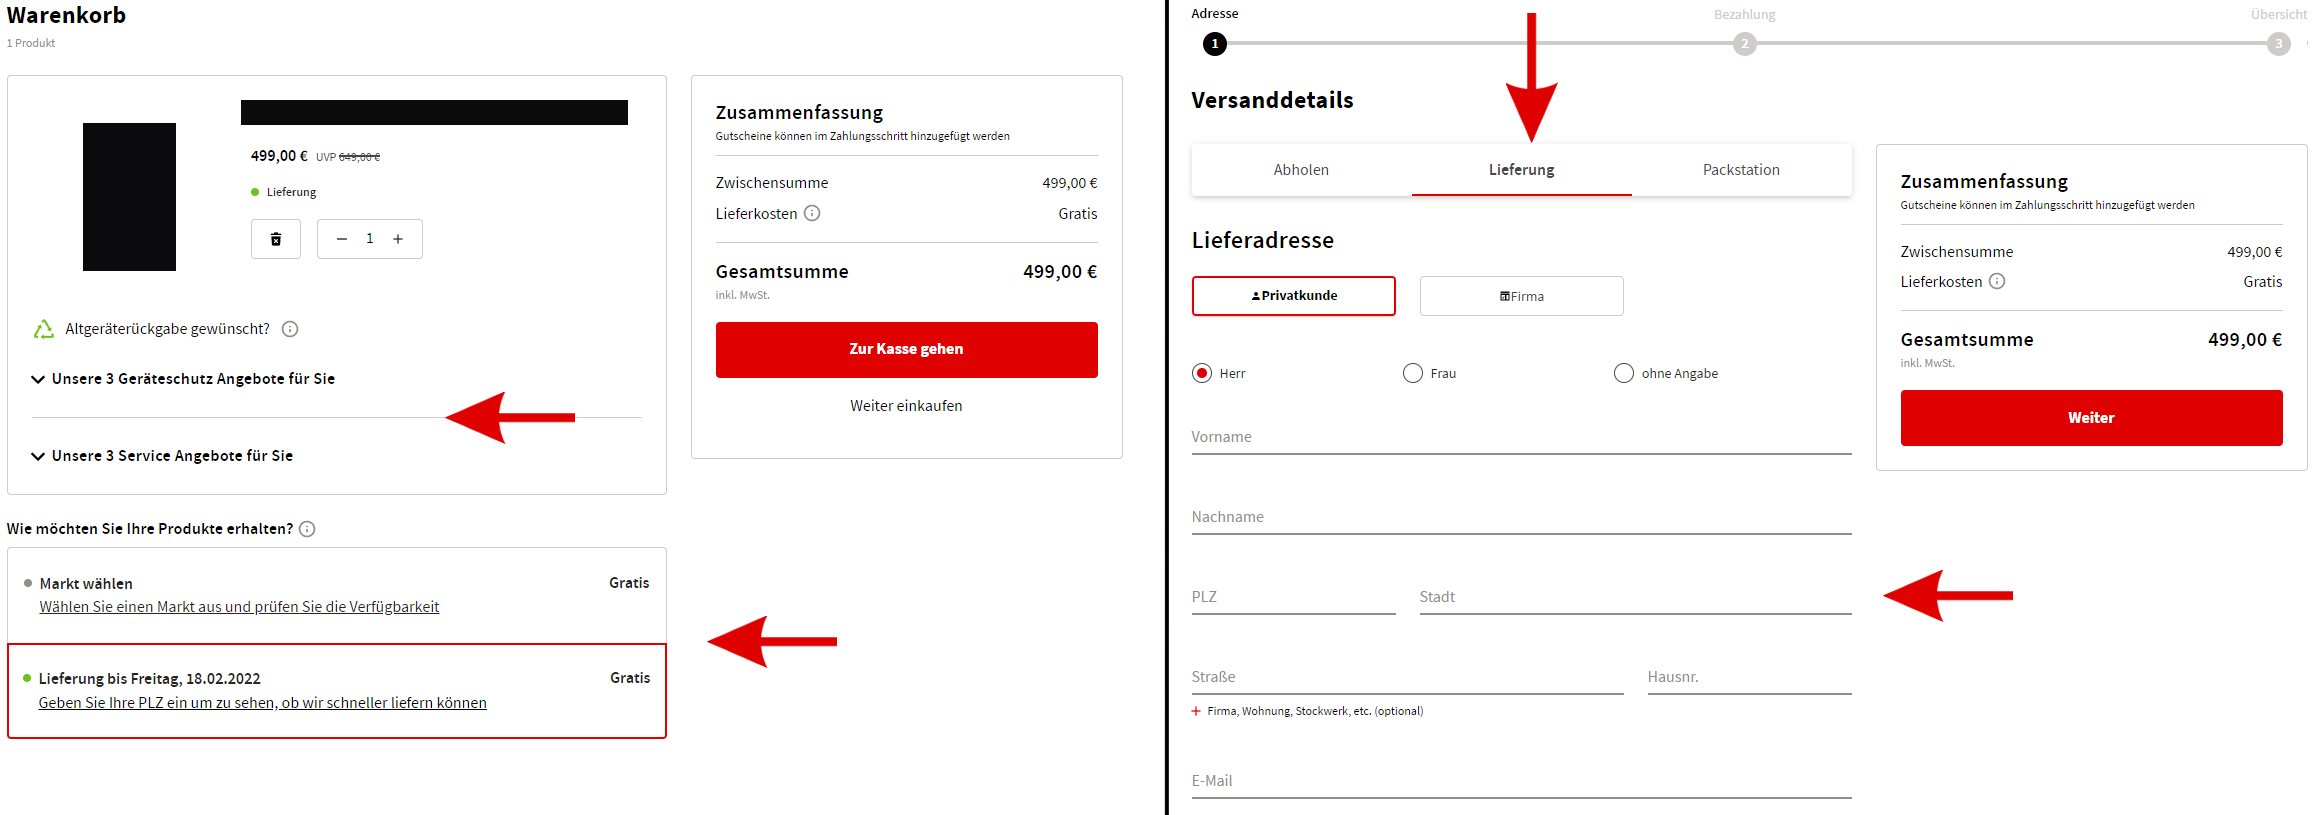
\includegraphics[width=\linewidth]{bilder/Checkout.png}}
	\caption{Aktueller Checkout-Prozess des Onlineshops von MediaMarkt.de}
	\label{fig:Checkout-Process}
\end{figure}

Eine Neukalkulation findet statt sofern die Anzahl der Produkte im Warenkorb oder die Lieferkosten manipuliert werden. Ersteres kann außerhalb des Warenkorbs geschehen oder durch Hinzufügen von Services während der Anzeige des Baskets. Ebenfalls kann die Fulfillment-Methode und Lieferadresse angepasst werden, wodurch sich die Lieferkosten ändern können. Schlussfolgernd existieren einige Anwendungsfälle in denen eine Transaktion über beide Aggregate hinweg notwendig ist.

\textbf{Gibt es Invarianten zwischen den Warenkorb und den Calculation-Result?}

Die Businessanforderung, dass das Berechnungsergebnis stets aktuell sein muss, wurde bereits gelockert. Verbleibend ist es zudem aus rechtlichen Gründen notwendig, eine Anpassung des Preises nach Initiierung des Zahlungsvorgangs zu verhindern. Dieses Problem kann allerdings nicht auftreten, da der Warenkorb selbst nicht mehr manipuliert werden kann, dementsprechend bleibt der Gesamtpreis ebenfalls unberührt. Weitere Voraussetzungen existieren zum jetzigen Zeitpunkt nicht, jedoch müssen eventuelle zukünftige Anwendungsfälle berücksichtigt werden, ansonsten kann die Flexibilität der Anwendung gefährdet sein. 

Zur Veranschaulichung dieses Aspektes wird die Auswirkungen einer neuen Regelung untersucht. Exemplarisch kann angenommen werden, dass der Gesamtpreis eines Warenkorbs nicht über 20.000€ liegen darf. In diesem Fall würde eine Manipulation der Elemente im Warenkorb auch eine Neukalkulation benötigen, wodurch die Abtrennung des Calculation-Results den Vorteil der verzögerten Berechnung verliert. Allerdings kann eine mildere Form dieser Richtlinie keinen negativen Effekt besitzen. Indem zum Beispiel die Prüfung erst beim Start des Bezahlvorgangs ausgeführt wird, da zu diesem Zeitpunkt beide Aggregates immer synchron sind und nachher keine Änderungen mehr erfahren können. Weitere erdenkbaren Businessanforderungen sollten berücksichtigt werden, bevor ein Neudesign der Applikation durchgeführt wird.

\textbf{Vorläufige Analyse der Bewertungskriterien}

\begin{itemize}[topsep=-2pt]
	\item \textbf{Komplexität: } { Die Implementierung kann ohne umfassendere Codeanpassungen realisiert werden. }
	\item \textbf{Performance: } { Zwar wird die Anzahl der Kalkulationen minimiert, jedoch steigen die Datenbankoperationen an, weil zuvor beide Objekte innerhalb einer Tabelle persistiert werden konnten, wodurch die Performance zweiseitig beeinflusst ist. }
	\item \textbf{Parallelität: } { Der Gesamtpreis wird nur als Wechselwirkung von Aktionen angepasst, sodass dieser Gesichtspunkt nicht bewertbar ist. }
	\item \textbf{Client-Freundlichkeit: } { Anhand der analysierten Fragestellungen ist die Anwenderfreundlichkeit davon abhängig, ob die Berechnungsergebnisse als Antwort von API-Aufrufen erwartet werden. Die Verwendung von Technologien wie GraphQL ermögliche die Rückgabe beider Aggregates und neutralisieren dieses Argument, jedoch beeinflussen wiederum wegen zusätzlichen Datenbankoperationen und Berechnungen die Performance. }
\end{itemize}

Grundsätzlich ist eine Abspaltung der Berechnungsergebnisse vom Warenkorb durchaus plausibel. Diese Vorgehensweise der Analyse kann analog auf verschiedene Anwendungsfälle durchgeführt werden, um weitere Teile des Baskets zu finden, welche separat agieren können. 

\subsection{Herausschneiden der Checkout-Daten aus dem Basket-Aggregate}

In dem Aktivitätsdiagramm \ref{fig:SL-Checkoutdata} wurde das Hinzufügen der Kundendaten, Zahlungsmethode und des Fulfillments beschrieben. Innerhalb eines API-Aufrufs soll eine Anpassung dieses Datenumfangs möglich sein. Das resultierende Webshop-Design in Bild \ref{fig:Checkout-Process} ist ein Hinweise darauf, dass diese Attribute eventuell aus dem Basket-Aggregat genommen werden können. Sie sind in der Ubiquitous Language als \emph{'Checkout-Daten'} betitelt und beinhalten Kundendaten, Fulfillment, Rechnungs- und Lieferadresse. Ähnlich zum vorgehenden Unterkapitel ist eine Untersuchung der Implikationen eines solches Aggregationsschnittes notwendig.

Nachteilig ist hier, dass dadurch die Value Objects zu einer Entity zusammengefasst werden müssen, da die Rolle des Aggregate Root nur durch Entities erfüllt werden darf. Deshalb wird die ursprüngliche eins-zu-eins Relation wiederum in der Datenbank als zwei separate Tabelle designt und zieht somit Performance-Einflüsse bei Abfragen beider Datensätze mit sich. Jedoch werden die Checkout-Daten in nahezu allen User Stories nur einmalig bearbeiten, sodass dieser Effekt minimal ausfällt.

Anpassungen an den Daten dürfen nur durchgeführt werden, wenn der Basket im Status 'open' ist. Aus diesem Grund muss bei jedem API-Aufruf zuvor der Zustand überprüft und der Warenkorb-Datenbankeintrag bis zum Abschluss der Bearbeitung gesperrt werden. Aufgrund von möglichen Race Conditions kann ansonsten beispielsweise die Initiierung des Bezahlvorgang auf invalide Checkout-Data stattfinden. Weiterhin können sich bei der Auswahl einer anderen Fulfillment-Methode die Lieferkosten ändern und folglich müssen die aktualisierten Preise des Warenkorbs persistiert werden. Hierbei stößt die Applikation auf eine Transaktion über zwei Aggregates und zugleich auf die vorher untersuchte Problemstellung.

Mithilfe dieses Designs ist der Basket leichtgewichtiger, geringere Datenmengen müssen bei Abruf transportiert werden und die Aufteilung der Aggregates spiegelt genauer die betroffenen Anwendungsfälle wider. Die genauere Bewertung der Performance und Komplexität findet in Verbund mit den vergangenen Aggregaten im nächsten Kapitel statt.

\comment{Bewertung hier? Unterkapitel ist bisschen kurz und der Aggregationsschnitt klingt sehr negativ belastet. Allerdings ist es schwer mehr zu schreiben als 'leichtgewichtiger' ohne sich im Kreis zu drehen...}

\section{Zusammenführung der vorgehenden Domain-Modelle}

Um einen möglichst unterteilten Aggregationsschnitt zu gewährleisten, wird auf Basis der vorgehenden Analysen ein kombiniertes Design erstellt, welches das \emph{Calculation-Result}, die \emph{Checkout-Data} und den \emph{Payment-Process} aus dem Basket in ihre eigenen Aggregates heraus hebt. Abbildung \ref{fig:VarD} zeigt das resultierende Datenmodell '\emph{Variante D}'. Eine Abspaltung der Basket-Items erfordert zu viele zusätzliche Datenbankoperationen und steigert die Softwarekomplexität weiter, wodurch diese nach wie vor unter dem Basket aufgehängt sind. Falls in zukünftigen Szenarien die parallele Bearbeitung der Warenkorbinhalte unerlässlich wird, kann eine Trennung der beiden Klassen voneinander in Betracht gezogen werden.  

\begin{figure}[htbp]
	\centering
	\includesvg[inkscapelatex=false, width=0.70\textwidth]{svg/VarD.svg}
	\caption{Aggregationsschnitt der Variante D}
	\label{fig:VarD}
\end{figure}

\subsection{Aktualisieren von veralteten Datenständen}

Ähnlich zu anderen Designvariationen benötigen viele Anwendungsfälle das gleichzeitige Laden und Bearbeiten mehrerer Aggregates. Beispielsweise beim Hinzufügen eines neuen Basket-Items ist die Neuberechnung des Payment-Processes und Calculation-Results notwendig. Gleichermaßen muss dieser Prozess angestoßen werden, wenn das Fulfillment in den Checkout-Daten bearbeitet und die Versandkosten des Warenkorbs sich dadurch ändern. Zur Abwicklung einer solchen Abhängigkeit sind mehrere Implementierungsmöglichkeiten denkbar.

Sollte die Kalkulationen erst bei Bedarf stattfinden, werden Zusatzinformation benötigt, um zu indizieren, dass der aktuelle Berechnungswert veraltet ist. Zu diesem Zweck wird ein Wahrheitswert (auch 'Flag' genannt) in den Basket und Checkout-Daten hinterlegt. Bei Zustandsänderungen, welche den Gesamtwert des Warenkorbs beeinflussen wird dieser auf 'wahr' gesetzt. Sobald ein Calculation-Result des dazugehörigen Baskets aus der Datenbank geladen wird, findet auch eine Neuberechnung statt, sofern der Wert 'wahr' ist, welche zugleich auch den Payment-Process aktualisiert. Dieses Vorgehen spart Berechnungszeit auf Kosten von zusätzlichen Datenbankoperationen ein. Die Komplexität und Fehleranfälligkeit der Software steigen hierbei an.

Andernfalls kann das CalculationResult bei jedem Abruf aus der Datenbank aktualisiert werden. Die Vor- und Nachteile sind im Vergleich zur vorherigen Lösung invertiert. Es sind mehr Kalkulationen notwendig, jedoch wird die Datenquelle entlastet. Sofern die Preisberechnung sich umfangreich gestaltet, sind Performance-Einbußen zu erwarten.

Alternativ kann unverändert zu \emph{Variante A} die Kalkulation sofort bei Datenänderungen geschehen. Allerdings werden die Aggregationsgrenzen überschritten und innerhalb einer Transaktion mehrere Aggregates bearbeitet. Dies stellt einen Zwischenweg der beiden vorgehenden Implementierungen dar.

In dem Proof-of-Concept sind erstere und letztere Vorgehensweise implementiert, um eine exemplarische Realisierung aufzuzeigen. 

\subsection{Dependency Injection von Services in Domain-Driven Design}

Umfangreiche oder nicht klar zuordenbare Funktionalitäten werde in Services ausgelagert. Die Reihenfolge der Serviceaufrufe ist durch den Anwendungsfall bereits vorgegeben, jedoch nicht in welcher Klasse diese stattfindet und wie die notwendigen Komponente an die Objekte übergeben wird. Verschiedene Implementierungen besitzen auch unterschiedliche Vor- bzw. Nachteile. Dieses Unterkapitel geht unter Beachtung von Dependency Injection auf einige Realisierungsmöglichkeiten genauer ein. 

\Gls{DI} ist eine spezielle Art des \acrlong{DIP}s. Hierbei initialisiert ein Framework erforderlichen Klassen durch ihren Konstruktor, indem die obligatorischen Parameter ebenfalls injiziert werden. Dadurch entsteht ein rekursives Muster bis schließlich alle Objekte erzeugt worden sind. Hiermit wird eine lose Kopplung der Module erreicht und eine Möglichkeit geschaffen, die konkreten Implementierungen anhand von Konfigurationsdateien auszutauschen. Eine Problematik dieser Vorgehensweise, welche auf inkorrektes Klassendesign hinweisen kann, ist die Bildung einer 'Circular Dependency' (dt. Zirkelbezug). Entsprechend der Grafik \ref{fig:circulardependency} tritt dies auf, sofern zwei Komponente voneinander abhängig sind. Das Framework versucht eine der beiden Klassen zu initialisieren, wobei im Konstruktor die verbleibende Klasse benötigt wird. Da diese jedoch ein Objekt der noch nicht erzeugen ersteren Klasse erwartet, entsteht ein ewiger Kreislauf von Konstruktoraufrufen. Eine Applikation mit einer Circular Dependency ist folglich nicht mehr ausführbar und die Eliminierung einer der Abhängigkeiten ist erforderlich. 

\begin{figure}[htbp]
	\centering
	\footnotesize
	\includesvg[width=\textwidth]{svg/circular dependency.svg}
	\caption{Darstellung einer Circular Dependency}
	\label{fig:circulardependency}
\end{figure}

Je mehr Abhängigkeiten eine Klasse besitzt, desto höher ist die Wahrscheinlichkeit des Auftretens einer Circular Dependency. Bei der konkreten Implementierung des Proof-of-Concepts stellte die Vermeidung einer solchen Situation teilweise eine Herausforderung dar.


\textbf{Steuerung des Programmablauf innerhalb von Domainservices}

Sofern mehrere Komponenten für die Durchführung eines Anwendungsfalles notwendig sind, fällt das Wissen über deren Aufrufreihenfolge in den Kontext der Domain. Deshalb sind Klassen außerhalb des Datenmodells mit mehreren Serviceaufrufen generell den Domainservices zuzuordnen. Im ersten Lösungsansatz wird der Programmablauf außerhalb des Aggregates durch einen Domainservice bestimmt. Das Codebeispiel \ref{lst:extract} implementiert beispielsweise einen Service zur Validierung einer Invariante. Dass zuvor eine Überprüfung der Validität einer Aktion stattfinden muss, stellt hier das Domainwissen dar. 

\begin{minipage}{\linewidth} % No pagebreak inside a minipage
	\begin{lstlisting}[caption={Bestimmung des Steuerflusses durch einen Domainservice}, label={lst:extract}, language=Kotlin]
class DomainService {
	
	function doStuff(Aggregate aggregate) {
		if (someService.isActionValid()) {     
			aggregate.doStuff()
		}
	}

}
	\end{lstlisting}
\end{minipage}

Die Eintrittswahrscheinlichkeit einer Circular Dependency ist gesenkt, da normalerweise die Domainservices sich nicht gegenseitig benötigen. Der größte Nachteil dieses Ansatzes liegt jedoch in der eingeführten Fehleranfälligkeit des Programms. Bei unvorsichtigen Codeanpassungen kann der Aufruf von 'aggregate.doStuff()' von anderen Abschnitten der Software ohne die vorgehende Validierung geschehen. Die Konsistenz des Aggregatzustandes ist somit gefährdet und damit verbundenen Qualitätsmerkmale werden geschwächt. Zur Verhinderung einer solchen Situation ist eine Verlagerung des Funktionsaufrufs in das Aggregate selber denkbar.


\textbf{Übergabe der Referenz an das Aggregate als Parameter}

Ein Aggregate sollte stets direkt alle wesentlichen Invarianten überprüfen, sodass die Ausführung von invaliden Aktionen unterbunden wird. Um dies zu gewährleisten, muss der Service innerhalb des Aggregates aufgerufen werden, weswegen dieser eine Referenz auf das gefragte Objekt benötigt. Dementsprechend wird in Figur \ref{lst:parameter} der Service als Parameter an das Aggregate übergeben.

\begin{minipage}{\linewidth} % No pagebreak inside a minipage
	\begin{lstlisting}[caption={Übergabe der Referenz an das Aggregate als Parameter}, label={lst:parameter}, language=Kotlin]
class DomainService {
	
	variable SomeService someService
	
	function doStuff(Aggregate aggregate) {
		aggregate.doStuff(someService)
	}
}

class Aggregate {
	// Kann nicht umgegangen werden, da Validierung direkt im Aggregate geschieht
	function doStuff(SomeService someService) {
		if (someService.isActionValid()) {
			...
		}
	}
}
	\end{lstlisting}
\end{minipage}

Dies löst das vorgehende Problem der Fehleranfälligkeit, jedoch wird die Funktionssignatur und das Aggregate aufgebläht. Grundlegend ist eine Abwägung notwendig, wann es sinnvoll ist, den Funktionsaufruf in das Aggregate mitaufzunehmen. Bei wichtigen Validierungen sollte diese Variante bevorzugt werden. Die Bewertung der Dependency Injection bleibt hier unverändert im Vergleich zur vorherigen Implementierung. Der Proof-of-Concept verwendet häufig diesen Ansatz, um Abhängigkeiten zu realisieren.

\textbf{Injektion der Service in ein Aggregate durch das Repository}

Weiterhin können auch zur Minimierung der Funktionsparameter die Services in das Aggregate hinein injiziert werden. Folglich halten die Aggregates selbst eine Referenz auf die jeweilig Klassen und rufen diese bei Notwendigkeit auf. Die Injektion muss bei Objekterzeugung geschehen, weshalb die Verantwortung bei den Repositories liegt. Im kurzen Beispielcode \ref{lst:injection} wird dieser Gedanke verdeutlicht.

\begin{minipage}{\linewidth} % No pagebreak inside a minipage
	\begin{lstlisting}[caption={Injektion des Services in ein Aggregate durch das Repository}, label={lst:injection}, language=Kotlin]
class Aggregate {
	
	variable SomeService domainService
	
	// Setzen des konkreten Service
	function inject(SomeService domainService) {
		this.domainService = domainService
	}
}

class AggregateRepository {
	
	variable SomeService domainService
	
	function load(Id id) returns Aggregate {
		variable aggregate = searchInDatabase(id)
		aggregate.inject(someService)
		return aggregate
	}
	
}
	\end{lstlisting}
\end{minipage}

Diese Methodik hat sich bei der Implementierung allerdings als problematisch erwiesen. Einerseits ist es fragwürdig, ob Datenklassen aus Entwicklersicht überhaupt Referenzen auf Services halten sollten, da weiter Abhängigkeiten erzeugt werden. Davon abgesehen erhöht sich stark die Wahrscheinlichkeit auf eine Circular Dependency innerhalb der Repositories, weil sie alle Services besitzen müssen, um diese den Aggregate zu übergeben. In \emph{Variante D} der Checkout-Software stehen die Aggregates in enger Bindung zueinander und benötigen zum Laden somit ihre gegenseitigen Repositories. Deshalb kann es bei Wechselwirkungen zwischen den Aggregates vorkommen, dass eine Circular Dependency auftritt.

\subsection{Performance-Analyse der Aggregationsschnitte unter Einsatz von Lasttests}

Damit eine genauere Aussage über die Performance von Variante A und D möglich ist, wird ein Lasttest mithilfe der Open-Source-Software 'JMeter' realisiert. Zuerst wurde hierfür ein gängiger Anwendungsfall definiert, welcher folgende Aktionen umfasst: Erstellen eines Baskets, dreimaliges Hinzufügen von Artikeln, Setzen der Checkout-Daten, zweimaliges Abrufen des Warenkorbs, Hinzufügen eines Payments und das Initiieren inklusive Durchführen des Bezahlvorgangs. Nach dem Vorbefüllen der Datenbank mit 1000 Datensätze wird anschließend dieser Prozessablauf in zehn parallelen Threads 'X'-mal durch die verschiedenen Aggregationsschnitte abgearbeitet. Zum Ausschließen von abweichenden Ergebnissen wird dies dreimal wiederholt. Die Auswertungen des Kapitels ist unter \ref{label:Lasttests} im Anhang zu finden.

\textbf{Bemerkungen zum Performance-Test}

Die Performance-Analyse dient lediglich als genereller Vergleich und weicht je nach Anwendungsfall, Hardware, Netzwerk und Softwareimplementierung ab. Zudem können weiterhin Optimierungsoptionen vorgenommen werden, wie die angepasste Einstellung des \Gls{Connection-Pool}s, das Einsparen von ganzen Datenbankoperationen durch Caching oder schnellere Kommunikation der Systeme untereinander. Anhand der Analyse sollen vorgehende Aussagen bewiesen und Argumente für das Fazit gebildet werden.

Zur simpleren Referenz der getesteten Varianten wird die Verwendung von MongoDB mit 'M' und von PostgreSQL mit 'P' abgekürzt. Weiterhin ist der Aggregationsschnitt D in die Untertypen 'F' bzw. 'C' unterteilt. Hierbei finden in der Abwandlung 'C' Nebeneffekte, wie die Neuberechnung des Gesamtpreises sofort statt, wohingegen in 'F' erst bei Abruf der jeweiligen Daten anhand von Flags erkennt wird, wann eine Neukalkulation notwendig ist. Folglich steht beispielsweise 'Variante D-PF' für den Aggregationsschnitt D mit einer PostgreSQL-Datenbank und Implementierung von Flags.

\textbf{Erster Testdurchlauf und hieraus ableitbare Aussagen}

Zu Beginn wurde der Proof-of-Concept für Variante A und D mitsamt ihren Abwandlungen implementiert und sachbezogene \acrshort{KPI}s (\acrlong{KPI}) anhand des obigen Testaufbaus ausgewertet. Das Ergebnis kann dem Anhang unter \ref{fig:performance-mongo} entnommen werden. Um die Konsequenz bei Verwendung einer relationalen Datenbank zu beobachten, wurde ebenfalls der Versuch mit einer PostgreSQL-Datenbank wiederholt. Die Auswertungen sind in Tabelle \ref{fig:performance-postgres} hinterlegt. Zum Präsentieren einer schnellen Übersicht wurde die durchschnittlichen 'Abläufe pro Sekunde' über einen Gesamtumfang von 10.000 Abläufen in der Grafik \ref{fig:PerformanceDefault} visualisiert.

\begin{figure}[htpb]
	\centering
	\footnotesize
	\includesvg[width=0.70\textwidth]{svg/Performance Default.svg}
	\caption{Performance-Ergebnisse aus dem ersten Testdurchlauf}
	\label{fig:PerformanceDefault}
\end{figure}

Mithilfe von Flags werden Neukalkulationen im Austausch für zusätzliche Datenbankoperationen eingespart, jedoch sind die eigentlichen Berechnungen des Warenkorbs in dem verkleinerten Proof-of-Concept trivial, weshalb zu beobachten ist, dass ein solches Vorgehen insgesamt zu einer geringeren Performance führt. In der aktuellen Live-Applikation kann aufgrund der komplexeren Berechnungsgrundlage dieser Ansatz allerdings weitaus performanter ausfallen. Negativ ist anzumerken, dass die Nutzung von Flags mit einem komplexeren Programmablauf einhergeht, da die Aktualisierung von Daten asynchron stattfinden. Bei der Implementierung von neuen Funktionen müssen stets die Wechselwirkungen zwischen den Wahrheitswerten und Businessprozessen beachtet werden, wodurch die Fehleranfälligkeit der Software steigt. Folglich sollten Flags nur in Betracht gezogen werden, sofern relevante Performance-Verbesserungen vernehmbar sind. Schlussendlich kann eine finale Aussage zwischen Variante D-C und D-F für die Produktivanwendung aufgrund der fehlenden Komplexität nicht getroffen werden.

In einem früheren Kapitel wurde die These aufgestellt, dass die Unterteilung von großen Aggregaten in kleinere unter Verwendung einer dokumentenorientierten Datenbank in geringeren oder sogar negativen Performance-Gewinnen resultieren kann, als beim Einsatz einer relationalen Datenbank. Diese Aussage ruht auf der Basis, dass mehr Datenbankoperationen bei einer MongoDB benötigt werden, sobald die Anzahl der Aggregates steigen, da zuvor alle Daten in einer einzelnen Collection abgespeichert werden konnten. Hingegen ist in relationalen Datenbanksystemen, aufgrund von Mehrfachbeziehungen und der Einhaltung von Normalformen, ein Aggregat bereits in mehrere Tabellen unterteilt und die weitere Abspaltung von Objekten führt zu insgesamt weniger neuen Relationen. In Tabelle \ref{fig:durationofexecution} wurde der Median über die Ausführungsdauer eines Anwendungsfalles pro Aggregationsschnitt gebildet und die Gesamtzahl der hierfür benötigten Datenbankoperationen aufgelistet. 

\begin{table}[htpb]
	\centering
	\begin{tabular}{ | >{\raggedright\arraybackslash}m{0.20\textwidth} || c | c | c | c | c | c | } 
		\hline
		Variante & A-M & D-MC & D-MF & A-P & D-PC & D-MF \\ 
		\hline
		Median-Dauer & 35ms & 31ms & 35ms & 56ms & 49ms & 56ms \\
		\hline
		Leseoperationen & 15 & 43 &  55 &  84 & 137 & 170 \\
		\hline
		Schreiboperationen & 15 & 27 & 28 & 108 & 98 & 127 \\
		\hline
	\end{tabular}
	\caption{Median der Ausführungszeit und Datenbankoperationen eines Durchlaufes}
	\label{fig:durationofexecution}
\end{table}

Der Performance-Unterschied beläuft sich auf 4 Millisekunden zwischen A-M und D-MC, sofern eine MongoDB als Datenbankmanagementsystem genutzt wird, wohingegen eine Einsparung von 6 Millisekunden bei einer PostgreSQL möglich ist. Dieser Effekt kann weiterhin deutlicher in kommende Testaufbauten beobachtet werden, worauf die vorliegende These gestützt wird. Aus den Daten ergibt sich allerdings die Frage, warum der Umbau zu Variante D überhaupt einen Performance-Gewinn mit sich bringt, obwohl dies mit mehr Datenbankoperationen einhergeht. 

Zum Speichern oder Laden von Datensätzen muss eine sogenannte De- bzw. \Gls{Serialisierung} stattfinden, damit die Daten richtig interpretiert werden können. Bei genauer Untersuchung der Datenbankzugriffe stellt sich heraus, dass dieser Vorgang aktuell den Großteil der Bearbeitungszeit in Anspruch nimmt, nicht wie zu vermuten die eigentliche Datenbankoperation. Deshalb sind die Variationen A insgesamt langsamer, da mehr Daten verarbeitet werden und somit zugleich die De-/Serialisierungsdauer erhöht wird. Diese Situation entsteht, da die Datenbank auf der gleichen Maschine wie die eigentliche Software ausgeführt wird. Die Kommunikation zwischen den Systemen ist nicht vom Netzwerk abhängig und ein Datenbankzugriff beläuft sich auf circa 1,5 Millisekunden. In den meisten Produktivumgebungen ist die Datenbank allerdings physisch getrennt, woraus Verzögerungen durch den Datentransport über das Netzwerk entstehen. Zur Simulation dieses Phänomens wird ein weiterer Performance-Test durchgeführt. 

\textbf{Aushängen der Datenbank in eine Cloud-Umgebung}

Damit eine ähnlichere Situation zur Produktivanwendungen geboten werden kann, wurde bei einem Cloud-Anbieter jeweils eine MongoDB und PostgreSQL in einem Frankfurter Datenzentrum mit 8 Gigabyte Arbeitsspeicher und 4 virtuellen Kernen angemietet. Der vorherige Testaufbau wird unter Verwendung dieser Datenspeichern wiederholt und tabellarisch dem Anhand unter \ref{fig:performance-database} hinzugefügt. Das Diagramm \ref{fig:PerformanceDatabase} bietet die dazugehörige grafische Auswertung.

\begin{figure}[htpb]
	\centering
	\footnotesize
	\includesvg[width=0.70\textwidth]{svg/Performance Database.svg}
	\caption{Performance-Ergebnisse bei Auslagerung der Datenbanksysteme}
	\label{fig:PerformanceDatabase}
\end{figure}

Die zusätzlichen Datenbankoperationen wirken sich nun stark auf die Performance des Proof-of-Concepts aus. Der mögliche Durchsatz von Variante A ist höher als der verkleinerte Aggregationsschnitt, da die De-/Serialisierung nur noch ein Bruchstück der Gesamtdauer ausmacht und die eigentliche Datenbankverbindung hingegen mehr Zeit in Anspruch nimmt. Die Differenz zwischen Variante A-M und D-MC beträgt hierbei durch das Netzwerk durchschnittlich 751 Millisekunden. Es muss beachtet werden, dass die Kommunikation mit den Datenspeicher aktuell die einzige Wartezeit der Applikation darstellt, wodurch der Einfluss auf die Performance unnatürlich hoch ausfällt. Zudem kann die Einbußen verringert werden, indem beispielsweise die Systeme physisch näher zusammenliegen oder eine dedizierte Verbindung mit der Datenbank über das Netzwerk hergestellt wird.


\textbf{Simulation von Wartezeiten bei Aufrufen von externen APIs}

Die Tatsache, dass Aufrufe an externe Systeme in zusätzlicher Wartezeit resultiert, wurde bis jetzt in den Performance-Test vernachlässigt. Aus der Analyse von Monitoring-Systemen der aktuellen Produktivanwendung konnten durchschnittliche API-Abrufzeiten gebildet und in die Applikation eingebaut werden. Im Mittel verbringt die Software 465 Millisekunden mit dem Warten auf Antworten von abhängigen Systemen. Der Testablauf wird auf Basis des ersten Tests inklusive der Wartezeiten-Simulation dementsprechend erneut durchgeführt. Die gemessenen Werte befinden sich in Tabelle \ref{fig:performance-delay} und im Balkendiagramm \ref{fig:PerformanceDelay}. 

\begin{figure}[htpb]
	\centering
	\footnotesize
	\includesvg[width=0.70\textwidth]{svg/Performance Delay.svg}
	\caption{Performance-Ergebnisse unter Beachtung der Wartezeiten bei API-Aufrufe}
	\label{fig:PerformanceDelay}
\end{figure}

Der mögliche Durchsatz sinkt bemerkbar und Unterschiede zwischen den Aggregationsdesigns verwaschen. Alle Aggregationsschnitte erfordern im Proof-of-Concept die gleiche Anzahl an API-Aufrufe. Sollte dies nicht der Fall sein, muss ein solcher Fakt ebenfalls mit in die Bewertung der Aggregates mit einfließen, weil sich unterschiedliche Wartezeiten und folglich Performance-Unterschiede ergeben. 


\textbf{Fazit aus dem Performance-Test}

Jegliche Art von Kommunikation mit externen Systemen gehen einher mit erheblichen Performance-Verluste der Software, da die eigentliche Datenverarbeitung in dem Proof-of-Concept minimal gehalten wurde. Der eventuelle Verlust von Performance muss anhand des konkreten Anwendungsfalles bewertet werden. Bei Systemen, in welchen zusätzliche 100 Millisekunden keine relevanten Auswirkungen auf die Businessprozesse haben, kann der Einfluss des Datenmodells auf die Performance in den meisten Fällen vernachlässigt werden. In produktiven Umgebungen fallen die Performance-Verluste zudem weitaus geringer aus. Letztendlich besteht jedoch die Tendenz, dass ein kleinerer Aggregationsschnitt im Kontext einer Checkout-Software in Kombination mit einer dokumentenorientierten Datenbank negative Auswirkungen besitzt.

\subsection{Bewertung des verkleinerten Aggregationsschnitt}

Die finale Evaluation ist ein Resultat der vorgehenden theoretischen Überlegungen, ein Vergleich mit anderen Varianten des Aggregationsschnitts und ihren tatsächlichen Implementierungen.

\begin{itemize}[topsep=-2pt]
	\item \textbf{Komplexität: } {Viele Prozesse benötigen zum Abfragen von externen Informationen oder für die Einhaltung von Invarianten mehr als ein Aggregat, wodurch zusätzlichen Funktionsaufrufe und Übergabeparameter eingeführt werden müssen. Dabei leidet die Übersichtlichkeit des Quellcodes. Dennoch ist es beispielsweise möglich durch Verwendung eines Kontextobjekts, auf welches überall in der Applikation Zugriff besteht, diese Auswirkungen einzudämmen, indem geladene Aggregate dort eingespeichert und abgerufen werden.
		
	Das Transaktionsmanagement gewinnt ebenfalls an Relevanz, sodass Datensätze so kurz wie möglich gesperrt sind. Sofern keine zeitgleichen Aufrufe auf dieselben Aggregates stattfinden, wirkt sich dies jedoch nicht bemerkbar auf die Performance aus. 
	
	Weiterhin muss für die Neuberechnung der Preise zum Abarbeiten von Nebeneffekten Flags eingeführt werden, sofern eine Vermeidung von extra Schreibprozesse angestrebt wird. 
	
	\emph{Insgesamt gewinnt die Applikation generell an Komplexität, welche je nach Realisierungsmethode stärker oder schwächer ausfallen kann.}}

	\item \textbf{Performance: } { \emph{Basierend auf die vorgehende Analyse ist ein Verlust von Performance vorhanden, da in der Live-Umgebung eine MongoDB verwendet wird.} }
	
	\item \textbf{Parallelität: } { Generell können zwei unterschiedliche Aggregates unabhängig voneinander bearbeitet werden. Als konkretes Beispiel ist die Bearbeitung von enthaltenen Artikeln und das Setzen von Checkout-Informationen gleichzeitig möglich. Eine tatsächliche Anwendung dieses Falles ist allerdings kaum denkbar. Sofern zusätzlich die Abspaltung der Basket-Items hinzukommt, gewinnt dieser Aspekt an Bedeutung. \emph{Die gewonnene Parallelität ist folglich nahezu vernachlässigbar bzw. nicht anwendbar.}}
	\item \textbf{Client-Freundlichkeit: } { Touchpoints erhalten als Antwort auf API-Anfragen in dieser Variante nur einen Teilaspekt des Baskets, denn andererseits müssten wieder alle Aggregate geladen werden, wodurch der Sinn einer Trennung verloren geht. Im Vorhinein findet mit den Clients eine Klärung über die erwarteten Antwortdaten mithilfe einer API-Vereinbarung statt, sodass diese ohne zusätzliche Anfragen weiterhin ihre Arbeitsprozesse abwickeln können. \emph{Letztendlich sind Clients bestenfalls nur neutral von der neuen Architektur betroffen.}}
\end{itemize}

Zusammenfassend existiert nur sehr beschränkt ein wirklicher Grund für die Anwendung von Variante D oder ähnlichen Aggregationsschnitten.